\chapter{实验}

\section{数据集}
\subsection{公开数据集}
本节中介绍本文使用的公开数据集。
\subsubsection{NeuralRGB-D数据}
NeuralRGB-D\cite{azinovic_neural_2022}提出了一个基于仿真的室内场景数据集,其中包含RGB和深度的准确数据。该数据提供了在 10 个合成场景的数据集,这些场景的真实几何和相机轨迹是已知的,因此可以提供隐式场方法的定量评估指标。其中,真实相机轨迹仅用于渲染和评估,而不用于重建。对于每一帧,作者使用 Blender渲染照片般逼真的图像,其后应用噪声和伪影,来模拟类似于真实深度传感器\cite{zabatani_intel_2020, zhang_microsoft_2012}。

\begin{figure}[ht]
    \centering
    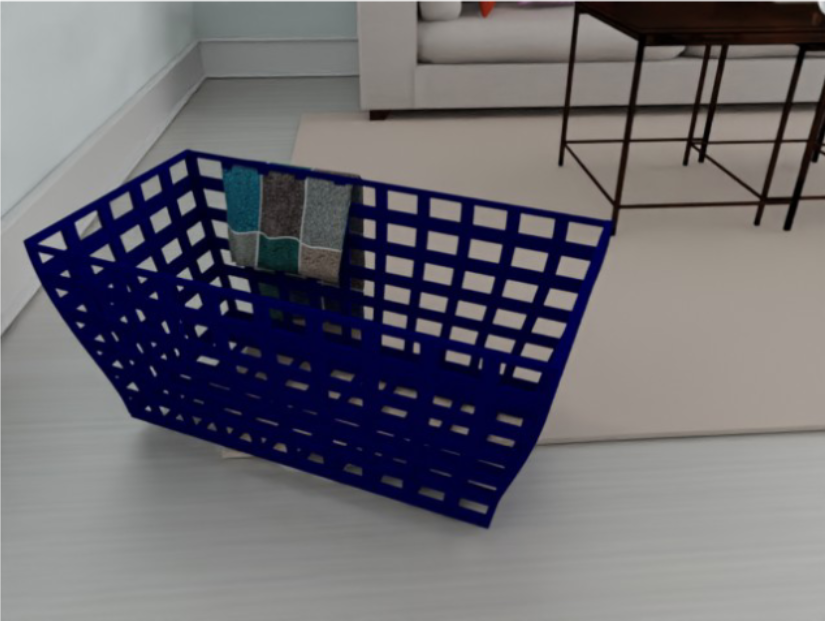
\includegraphics[width=0.6\textwidth]{undergraduate-thesis/images/experiments/neural-rgbd dataset.png}
    \caption{NeuralRGB-D\cite{azinovic_neural_2022}中的场景thin-Geometry示例图片}
    \label{fig:exp-neural-rgbd-data}
\end{figure}

\begin{figure}[ht]
    \centering
    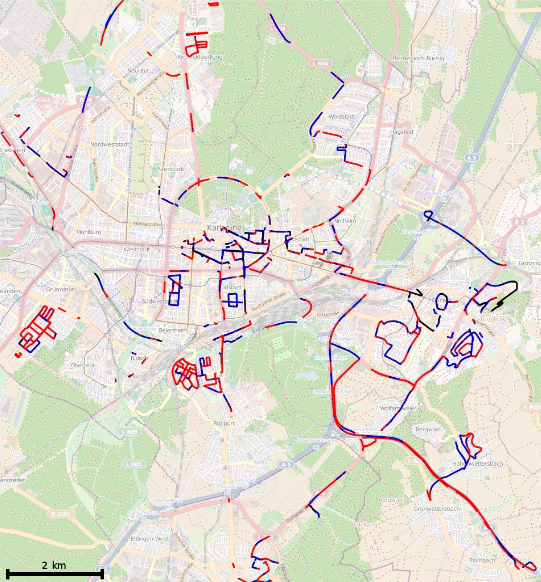
\includegraphics[width=0.8\textwidth]{undergraduate-thesis/images/experiments/kitti-map.png}
    \caption{KITTI数据集所覆盖的地图范围}
    \label{fig:exp-kitti-map}
\end{figure}

\subsubsection{KITTI数据集}
KITTI数据集\cite{geiger_are_2012,geiger_vision_2013}是是在德国卡尔斯鲁厄及其周边地区行驶时从移动平台\ref{fig:exp-kitti-platform}记录的。它包括来自组合 GPS/IMU 系统的相机图像、激光扫描、高精度 GPS 测量和 IMU 加速度。该数据集的主要目的是推动以自动驾驶为目标的计算机视觉和机器人算法的发展。在本文中,我们使用其中包含动态物体较多的片段,以验证本文所提出的场景图方法在重建复杂动态场景时的性能。
\begin{figure}[ht]
    \centering
    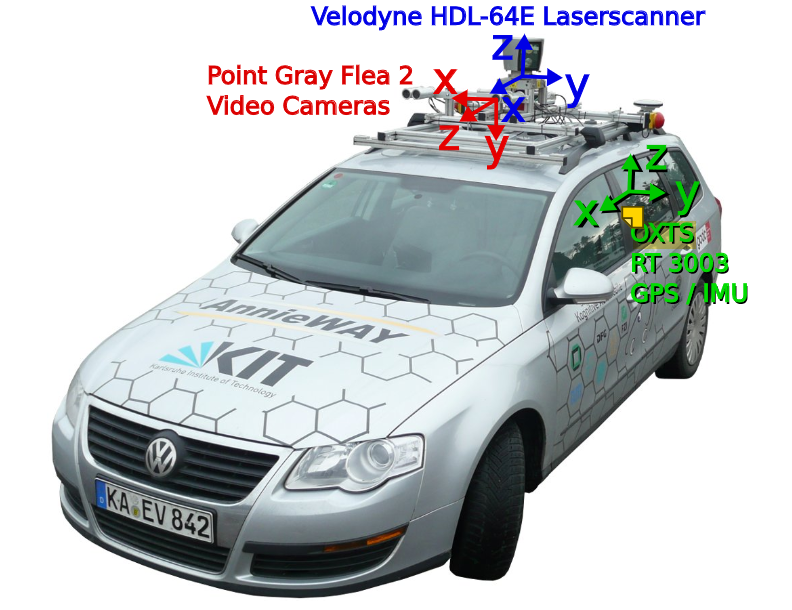
\includegraphics[width=0.8\textwidth]{undergraduate-thesis/images/experiments/kitti-platform.png}
    \caption{KITTI数据集的采集平台}
    \label{fig:exp-kitti-platform}
\end{figure}

图\ref{fig:exp-kitti-map}显示了KITTI数据集在德国卡尔斯鲁厄大都市区记录的 GPS 轨迹。颜色编码 GPS 信号质量:红色表示已使用 RTK 校正以最高精度记录,蓝色表示没有校正信号。由于没有可用的 GPS 信号,黑色部分已从数据集中排除。
KITTI数据集中提供了场景中动态物体的边界框位姿,如图\ref{fig:exp-kitti-objpose}所示。对于参考相机视野内的每个动态对象,KITTI以 3D 边界框轨迹的形式提供标注,以 Velodyne 坐标表示。数据集中定义了“汽车”、“货车”、“卡车”、“行人”、“人(坐着的)”、“骑自行车的人”、“电车”和“其他”(例如,拖车、赛格威)等多个物体类别。

\begin{figure}[ht]
    \centering
    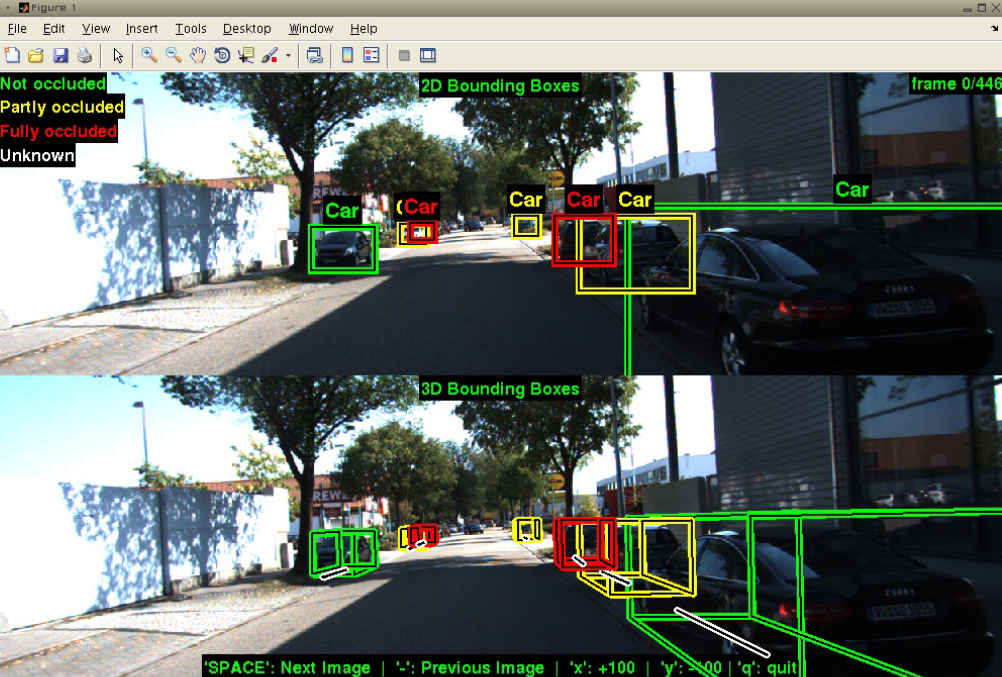
\includegraphics[width=\textwidth]{undergraduate-thesis/images/experiments/kitti-objects.png}
    \caption{KITTI中动态物体轨迹位姿标定可视化}
    \label{fig:exp-kitti-objpose}
\end{figure}



\subsection{本文提出的数据集}
\subsubsection{仿真数据集}

\subsubsection{真实数据集}

\section{混合隐式场景重建}


\section{场景图重建}

\section{体渲染方法}

\section{消融实验}

\section{本章小结}